
\subsection{1.23 Соединения переходных металлов 7 группы. Геометрия молекул в зависимости от природы лигандов, их электронное строение, способы получения и химическое поведение.}
\begin{itemize}
	\item $Mn$: $(+1), +2, +3, +4, (+5), +6, +7$	
	\item $Tc$: $(+2), +3, +4, +5, (+6), +7$
	\item $Re$: $(+2), +3, +4, +5, +6, +7$
\end{itemize}
В природе 
\begin{itemize}
	\item $Mn$: \\
	$MnO \cdot nH_2O$ - пиролюзит, $MnCO_3$ - родохрозит, $Mn_2O_3 \cdot nH_2O$ - манганат.
	\item $Tc$: \\
	нет стабильных изотопов
	\item $Re$: \\
	редкий и рассеянный  элемент, извлекается из молибденовых руд
\end{itemize}
Свойства:
\begin{itemize}
	\item $Mn$:
	\begin{itemize}
		\item $+ N_2 = Mn_3N_2 $
		\item $+ H_2O = Mn(OH)_2 + H_2 $
		\item $+ HCl = MnCl_2 + H_2 $
		\item $+ KOH \not =  $
		\item $+ H_2 \not = $
		\item $+ F_2  = MnF_3$
		\item $+ O_2 = Mn_3O_4 $
		\item $+ C = Mn_3C \quad Mn_7C_3 \quad Mn_5C_2 $
		\item $+ Cl_2 =  MnCl_2 $		
	\end{itemize}
\end{itemize}
$Mn^0$ расстворяется с образованием комплексов:
\begin{align*}
Mn + 6 NaCN + \frac12 O_2 + H_2O &= Na_4\left[Mn^{+2}(CN)_6\right] + 2NaOH \\
Mn + 6 NaCN + H_2O &= Na_5\left[Mn^{+1}(CN)_6\right] + NaOH + \dfrac12 H_2
\end{align*}
\begin{figure} [H]
	\centering {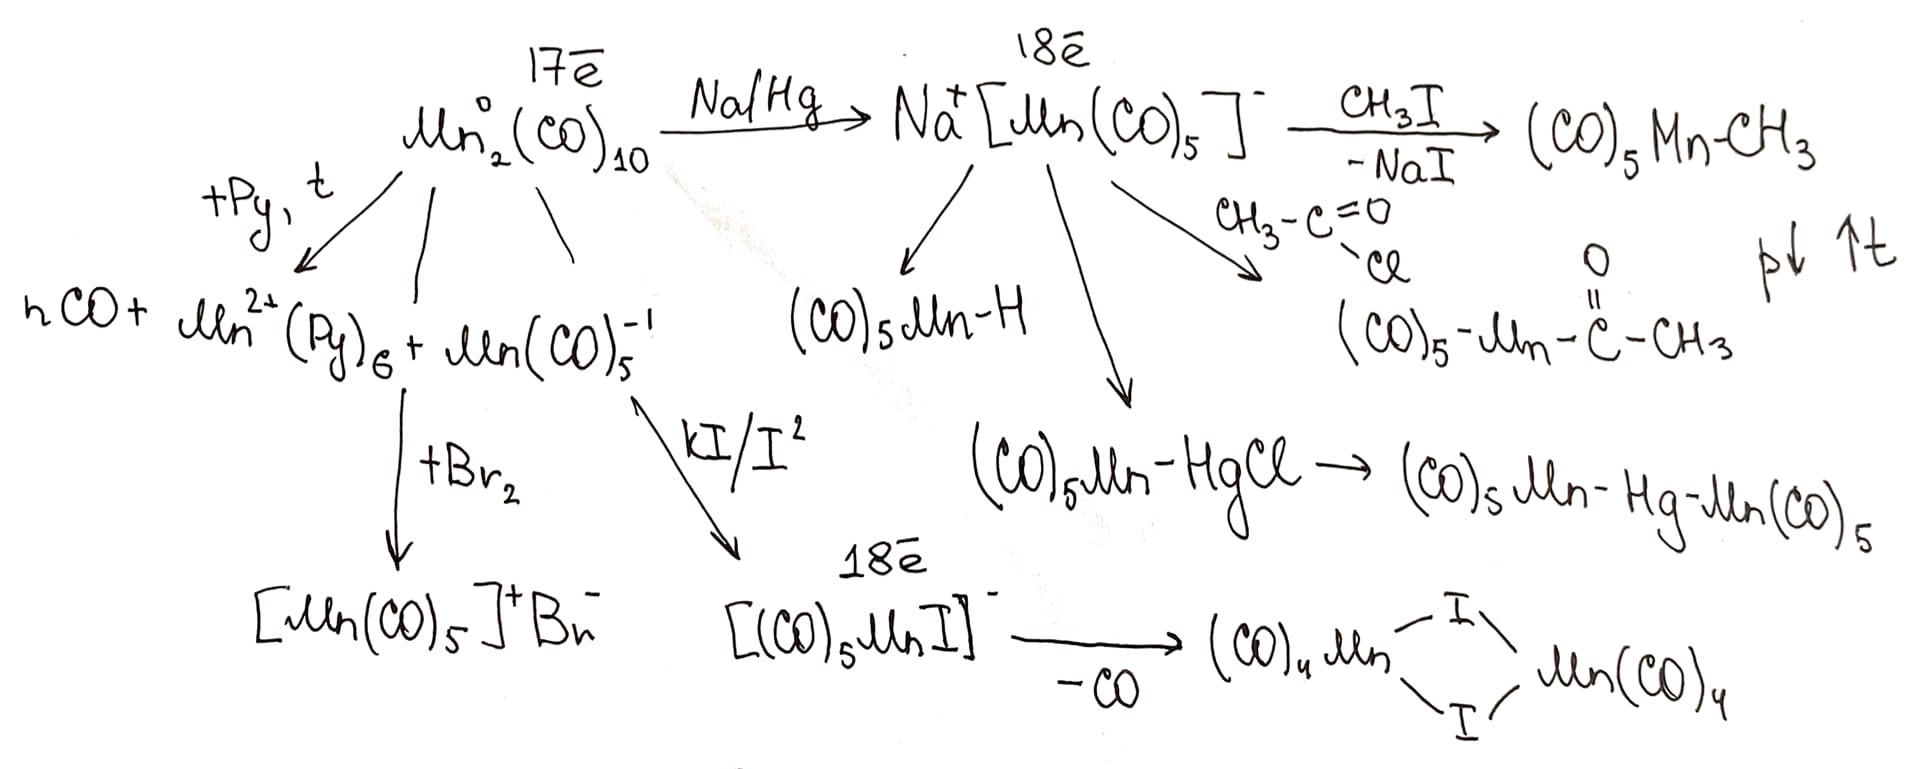
\includegraphics[scale=0.25]{zz1}}
\end{figure}
Свойства:
\begin{itemize}
	\item $Tc, Re$:
	\begin{itemize}
		\item $+ KOH \not = $
		\item $+ HCl \not = $
		\item $+ HNO_3\text{(к)} = HReO_4 + NO + H_2O$
		\item $+ H_2 \not = $
		\item $+ S  = ReS_2$
		\item $+ Cl_2 = ReCl_5$
		\item $+ F_2 = ReF_6$
		\item $+ O_2 =  Re_2O_7$		
	\end{itemize}
\end{itemize}
\textbf{Степень окисления $+1$} \\
$Mn^{+1}$ стабилизируется $\pi$-акцепторными $L$:
\[
Na_5\left[Mn^{+1}(CN)_6\right] \quad \left[Mn^{+1}(CO)_5\right]Br
\]
\textbf{Степень окисления $+2$} \\
$Mn^{+2}$ похож на $Mg^{+2}$, основный характер \\
Наиболее устойчивы оксо- и фторокомплексы 
$MnSO_4 + 6 H_2O = \left[Mn(H_2O)_6 \right]SO_4$ - октаэдр \\
$4KF + MnF_2 = K_4\left[MnF_6 \right]$ - октаэдр \\
$K_2\left[MnBr_4 \right]$ - тетраэдр \\
$\left[Mn(H_2O)_6 \right]^{2+} \quad \left[MnF_6 \right]^{4-} $
\begin{figure} [H]
	\centering {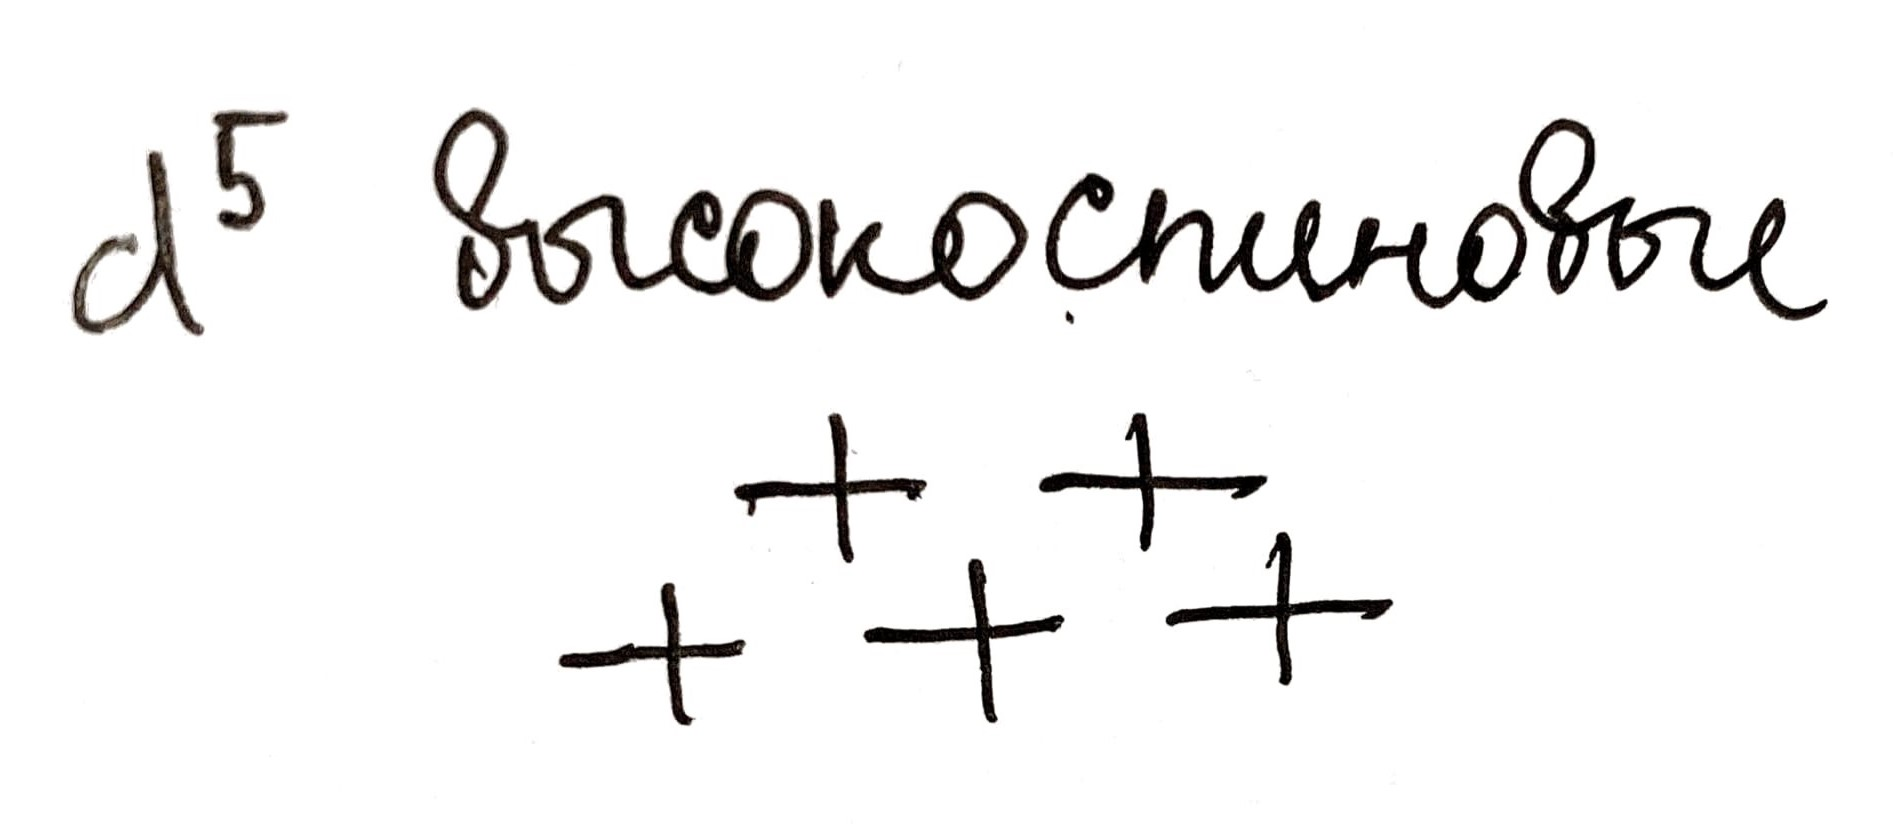
\includegraphics[scale=0.1]{zz3}}
\end{figure}
$ \left[Mn(CN)_6 \right]^{4-} $
\begin{figure} [H]
	\centering {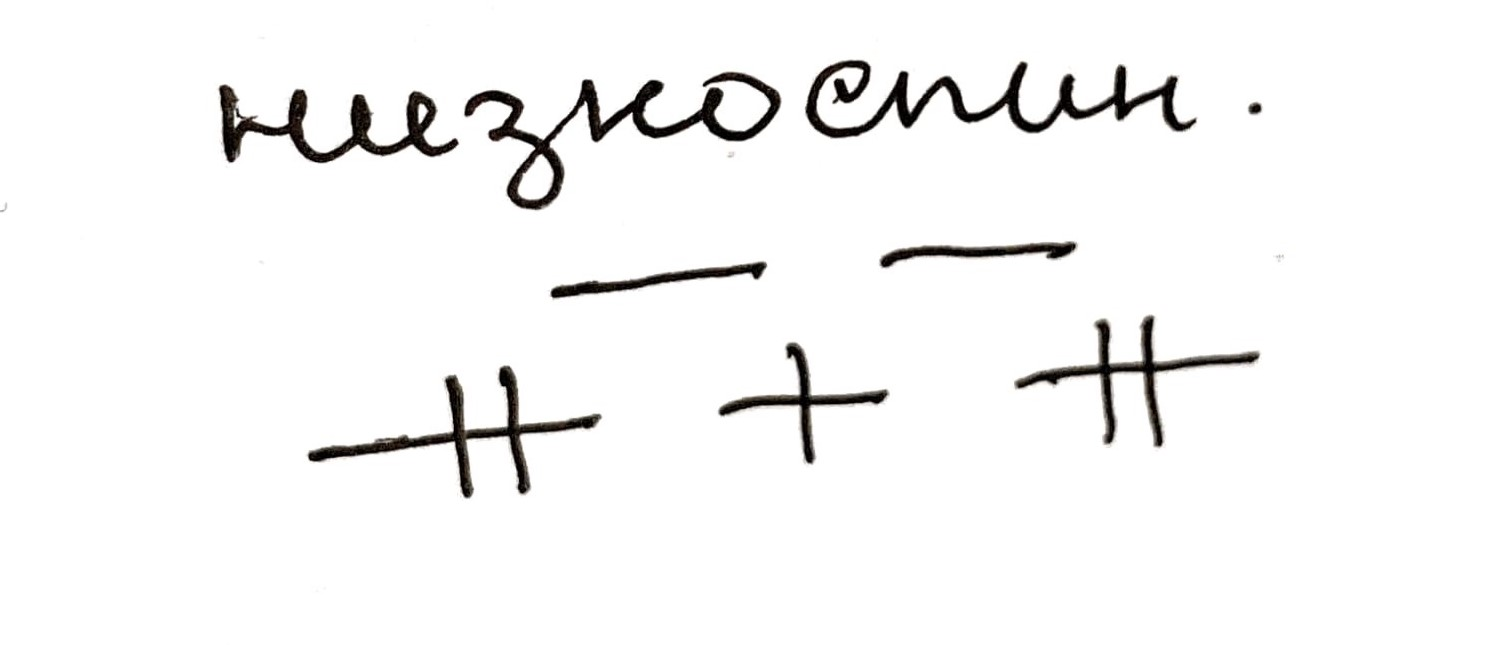
\includegraphics[scale=0.1]{zz2}}
\end{figure}
В низших степенях окисления $Re$ образует кластеры \\
\textbf{Степень окисления $+3$} \\
$\left[Mn(H_2O)_6 \right]^{2+}$ не стабилен, диспропорционирует \\
$Mn^{+3}$ можно стабилизировать $F^-, PO_4^{3-}, C_2O_4^{2-}$ \\
$\left[Mn(C_2O_4)_3 \right]$ - устойчивый хелатный комплекс \\
$\left[MnF_6 \right]^{3-}$ - октаэдрический, эффект Яна-Теллера: 
\begin{figure} [H]
	\centering {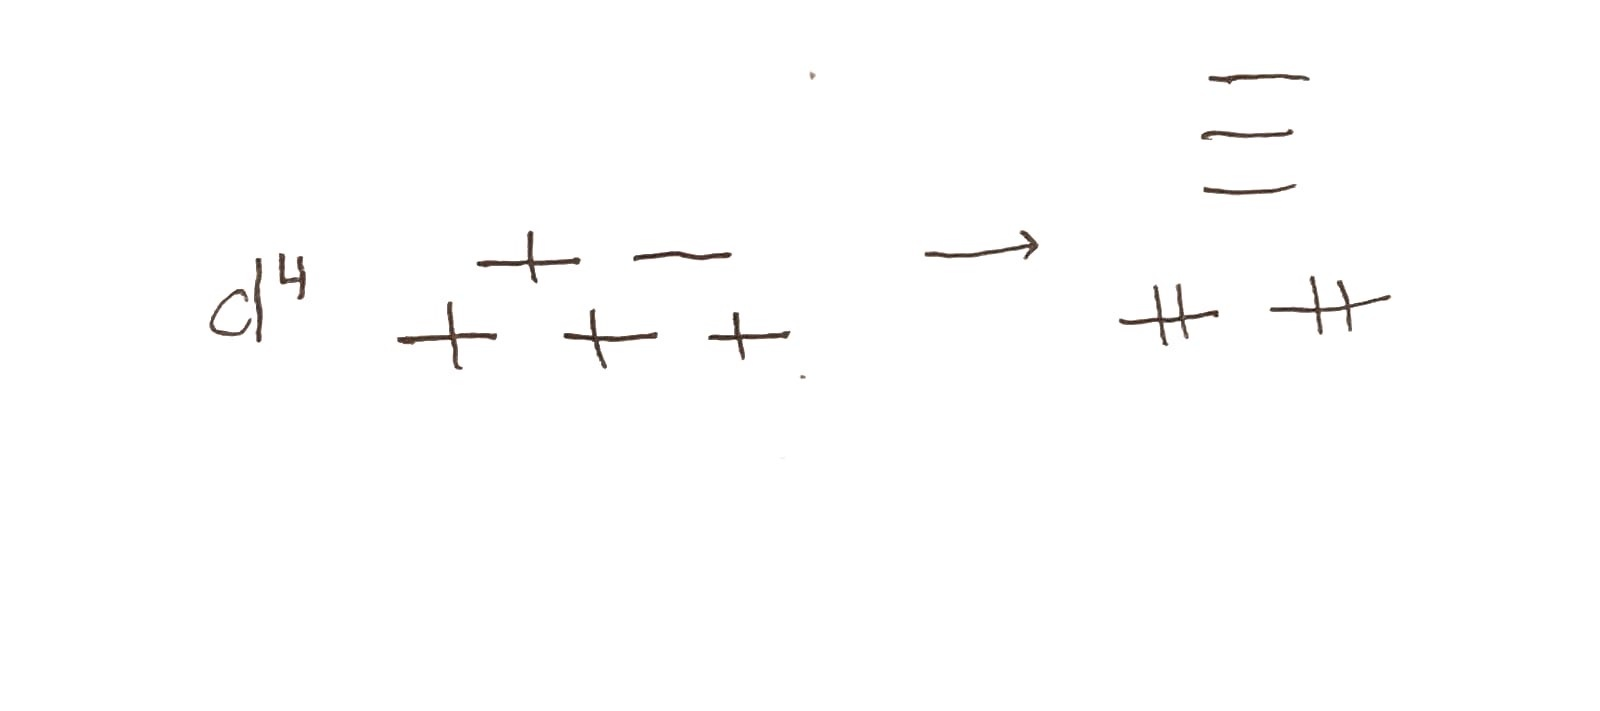
\includegraphics[scale=0.15]{zz4}}
\end{figure} 
Анионы $MnF_5^{2-}$ и $MnF_4^{-}$ имеют октаэдрическую структуру с искажением Я-Т. \\
$ReCl_3, ReCl_4$ - тримеры \\
$\left[MnCl_5 \right]^{2-} $ - квадратная пирамида. \\
Стабилизация $Mn(III)$:
\begin{align*}
KMnO_4 + 6 KF + 8HCl &= K_3\left[MnF_6 \right] + 4H_2O + 4KCl \\
KMnO_4 + H_2SO_4 + H_2O_2 &= K\left[Mn(SO_4)_2 \right] + 2O_2 + 4H_2O \\
KMnO_4 + 8Hcl + 2 KCl &= K_3\left[MnCl_6 \right] + 2Cl_2 + 4H_2O
\end{align*}
Хелатные более устойчивы:
\[
3MnO(OH) + 3H_2C_2O_4 + 3K_2C_2O_4 = 2K_3\left[Mn(C_2O_4)_3 \right] + 4H_2O
\]
Низкоспиновые:
\begin{align*}
2K_4\left[Mn^{+4}(CN)_6 \right] + H_2O_2 &= 2K_3\left[Mn^{+3}(CN)_6 \right] + 2KOH \\
K_3\left[MnF_6 \right] + 6KCN &= K_3\left[Mn(CN)_6 \right]	+ 6KF
\end{align*}
\textbf{Степень окисления $+4$} \\
$MnF_4$ - тетрамеры \\
$Mn^{+4}$ легко гидролизуется \\
Комплексы $Mn^{+4}$ (самые устойчивые - фторидные):
$\left[Mn(CN)_6 \right]^{2-}$ \\
\begin{align*}
MnF_2 + F_2 + KF &= K_2\left[MnF_6 \right] \\
K_2\left[MnF_6 \right] + SbF_3 &= K\left[SbF_6 \right] + MnF_2 + KF
\end{align*}
$TcO_2, ReO_2$ не растворяются в $H_2O$, в щелочах и в кислотах. \\
\textbf{Степень окисления $+5, +6$} \\
$\left[MnO_4 \right]^{2-}, \left[MnO_4 \right]^{3-}$ - существуют в щелочи, неустойчивы, диспропорционируют \\
Гидридные комплексы: $ TcH_9^{2-}, ReH_9^{2-} $
\begin{figure} [H]
	\centering {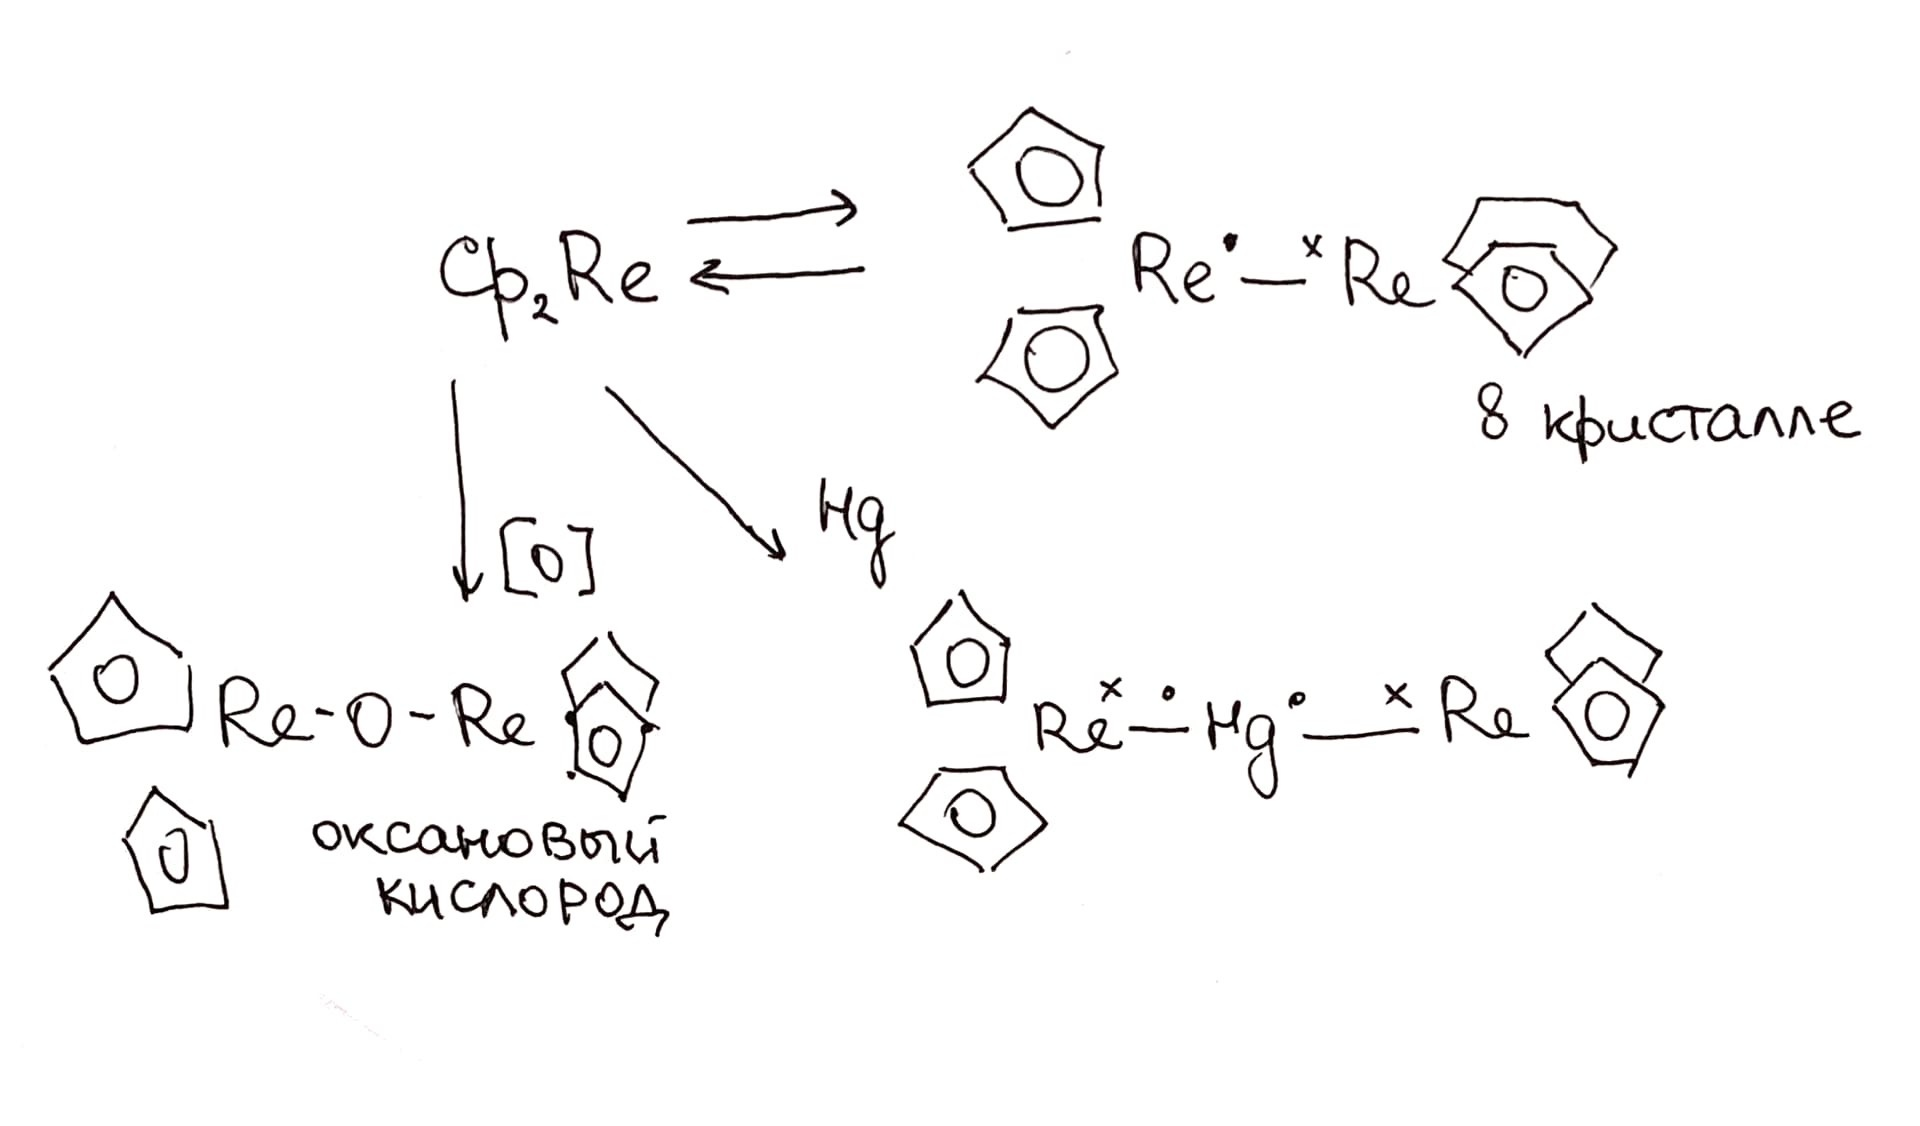
\includegraphics[scale=0.17]{zz5}}
\end{figure}

